\section{Background and related work}
\label{sec:background}
There exists an extensive literature on query
optimization. Here, we point to some of the fundamental papers and then describe MongoDB (the system we study in this paper) and how its \approachName query optimization is performed.



%%%%%%
%% Query Optimization Concepts
%%%%%%%%%%%%%%%%%%%%%%

\subsection{Query Optimization Architecture}

A vital factor in the spread of relational database technology was the support for declarative queries, in which a user expresses a query indicating {\it what} information is needed and the system then discovers {\it how to} execute the query, that is, what steps to take to retrieve that information from what is stored~\cite{Codd70}. Declarative queries have remained important also with other data models, such as object and document data. In general, a given query will have many execution plans (the details will depend on physical structures such as indexes), and these plans will differ greatly in performance. For declarative queries to be workable, the database management system must be able to optimize, that is, find an execution approach which is not only correct in retrieving the specified information, but also runs rapidly.

Although some early commercial systems used pure heuristics to choose the execution plan for a submitted query, the dominant approach is cost-based optimization, invented by Selinger and colleagues for System~R~\cite{SelingerACLP79}. The essential work of a cost-based optimizer is (i) generate a variety of \emph{candidates}, which are execution plans each of which would calculate the correct results for the given query, (ii) estimate the cost each candidate plan will incur when it runs, and (iii) choose to actually execute the plan, among those considered, whose estimate cost is lowest. Cost-based optimization is now industry standard practice~\cite{lahdenmaki2005relational}.

Research has continued apace, both in industry and academia, to improve the design of query optimizers.

\subsection{Candidate Plan Generation} \label{sec:candidate-plan-generation}
For complicated queries, there are a very large number of execution plans that produce the correct results. The plans can vary logically (for example, in which order joins are done, whether selection happens before or after a join, etc.) and physically (e.g., which index is used to find records, which join algorithm is used). The System~R optimizer~\cite{SelingerACLP79} restricted its attention to joins performed in a particular set of sequential patterns. The generation of potential logical plans by successively applying transformations was introduced by Freytag~\cite{Freytag87} and Graefe~\cite{GraefeD87} and used in IBM's Starburst project~\cite{HaasFLP89, PiraheshHH92}.  Later, Graefe extended this to a unified view in which logical and physical choices were treated together to generate potential plans~\cite{Graefe95a}.

\subsection{Cost Estimation}
The cost one estimates is a measure of the resources consumed in calculation; traditionally, for a disk-based database management system, the dominant cost is bringing pages from disk to memory or vice versa. To estimate the cost of an execution plan, one proceeds from estimates of the cost of each operation (e.g. join, select) within the plan. The cost of a step depends on the physical structure and especially on the cardinality of the inputs and outputs of the step. For base collections, cardinality is clear, but subsequent operations take as inputs the results of prior calculations, and so estimating the cardinality requires estimating the selectivity of predicates, the number of distinct values in an attribute, the probability that items will match in a join, etc. Many techniques have been proposed for estimating specific operations such as projection, range, join, and aggregation~\cite{ahad1989estimating, HaasNSS96, PoosalaIHS96, MarklMKTHS05}. Estimates are often based on statistics kept in the database or calculated dynamically by sampling~\cite{olken1995random}.

The cost estimate for a plan is very sensitive to errors in the cardinality estimates, so several researchers have tried to achieve \emph{robust} planning, where the plan choice works well even if the estimates are mistaken. One approach is to include a measure of uncertainty in each estimate~\cite{babcock2005towards}, and then choose a plan that is good throughout the likely range of estimates. Another is to check while the chosen plan is executing and to stop and re-optimize if the reality differs too much from what was estimated~\cite{markl2004robust}. These ideas have been combined~\cite{babu2005proactive}.

%In database systems, cost models are used for enhancing the efficiency of query optimization. Database query optimizers attempt to determine the most efficient way to execute a given query by considering all possible query plans. The question of how to select optimal query plans among all alternatives arises. An important assumption made on an optimal query plan is that it consumes fewer resources and time when less data is need to be  processed. \cite{cammert2006cost}.

%It is not immediately clear, among various sequences of operations, which one requires the least amount of time and resources. To resolve this problem, cost models rely on statistics about the distribution of data, and based on this consider the estimated costs of executing the algorithms and of accessing resources. In summary, cost models estimate multiple cost factors involved in query execution to facilitate the selection of optimal query plans \cite{olken1995random}.


%\subsection{Cardinality Estimation and Selectivity Estimation}


%Cardinality is used as an input parameter of the cost model. Therefore, improving cardinality estimation leads to more accurate cost models, thereby obtaining a faster execution plan.Traditional query optimizers perform a phase of cost-based plan comparison to identify the query plan with the lowest cost (i.e. the most efficient query plan). Since page I/O cost often dominates, it is crucial to estimate the cardinality of intermediate results. To achieve this, cost-based query optimizers use selectivity estimation to predict the result size of each query predicate. 

%To estimate result cardinality, traditional database systems store statistical information about the dataset using histograms, sampling and  parametric techniques.  In general, statistics are hard to maintain while supporting heavy write loads. And all variations of estimation approaches suffer from small  errors generated during estimation that might lead to a suboptimal query plan being chosen.

%the majority of RDBMS (relational database management system) query optimizers  mathematically model the cost for each alternative query plan and select the one with the lowest cost as the execution plan \cite{lahdenmaki2005relational, Ora15, Valentin:20005d5}. The cost evaluation process crucially relies on cardinality estimation which predicts the number of rows (result cardinality) that fulfils the condition of each predicate in the query \cite{Chaudhuri:1998478, babcock2005towards}.

%Research on query optimization has a long tradition, some research focuses on improving selectivity estimation (the percentage of total rows a predicate will select), cardinality estimation (the number of rows in a given selection) and dynamic re-evaluation invoked during runtime \cite{ ahad1989estimating,lahdenmaki2005relational,babu2005proactive, chaudhuri2008pay}. 
%One important theme has been to avoid sub-optimal query plans as much as possible. Those contributions include creating visualization tools for query plan costs and the re-design of performance benchmarks for evaluating the robustness of query optimizers \cite{reddy2005analyzing, babcock2005towards}. 
%These prior works enlightened us, yet we draw the following distinction between those previous efforts and our own. Consequently, nowadays the majority of commercial databases use cost-based query optimization techniques. 

\subsection{Optimizer Implementation and Use}
Graefe and others have emphasized the importance of modularity and extensibility of the optimizer~\cite{Graefe94, Graefe95a}. An important theme has been to allow parallel execution in the optimizer~\cite{WaasH09, SolimanAREGSCGRPWNKB14}. 
Chaudhuri and colleagues at Microsoft and Lohman and others at IBM pioneered the use of the cost estimator component as a tool to recommend better physical structures, e.g., deciding which indexes to create~\cite{Chaudhuri:1998478, Chaudhuri:20049cd, Valentin:20005d5, Agrawal:2005dff, chaudhuri2008pay}.

Recent work has focused on learning from dynamic query execution for adaptive code generation to avoid adding complex, specialized query execution techniques to support diverse hardware~\cite{Gubner22}; and using reinforcement learning to adaptively change query plans during execution~\cite{Trummer21}. MongoDB's \approachName approach was designed before this work, and while it is simpler, it has been in widespread use for many years and thus is still of interest.

\subsection{Evaluating Query Optimization}
While much of the literature has taken an engineering approach, designing better ways to do optimization, there has also been work that is scientific in style, looking at how to evaluate the quality of a given optimizer. Our paper follows this tradition. For cost-based optimizers, there has been study of how accurate the estimates are, by comparing the estimated cost with the measured cost when a plan is run~\cite{GuSW12, LeisGMBK015}. This does not of course apply to MongoDB, since \approachName does not use cost estimates. Another aspect of evaluation is to find a suitable set of queries on which to test the optimizer. In this paper we use simple conjunctive queries with two range predicates, but more complex queries are important in practice, and some systems have generated random queries with a mix of predicates and joins, eg~\cite{StillgerF95, WaasG00}. Our work has been most influenced by the work of Haritsa and colleagues, whose focus is on understanding which plan is chosen for each query, especially as selectivity varies. The Picasso tool~\cite{reddy2005analyzing, Haritsa10} introduced plan diagram visulization, which is one of the displays we use here. This led to a new goal for an optimizer: to be stable (that is, to have a plan that works well not just for the given query, but also for nearby ones)~\cite{AbhiramaBDSH10}.

%%%%%%
%% MongoDB 
%%%%%%%%%%%%%%%%%%%%%%
\subsection{Document Data Model}
MongoDB is a document-oriented database designed for ease of development and scaling. A MongoDB database stores collections of documents. MongoDB documents (the equivalent of records in a relational DBMS) do not need to have a schema defined beforehand \cite{chandra2015base, mongodb_2019}. Instead, the fields in each document can be chosen on the fly.  This flexible design allows developers to represent hierarchical relationships, to store arrays, and other more complex structures simply.

% [Michael] I'm inclined not to over-sell.
% The  design of MongoDB environments are very scalable. Companies across the world have deployed clusters running more than a hundred nodes with around millions of documents within the database.

The key components of the MongoDB data model design are the database, collection, document, and cursor \cite{banker2011mongodb}.
Table \ref{table:terms} shows the relationship of RDBMS terminology with MongoDB. 

% [Michael] I think we could cut this table for space without losing much
\begin{table}[htb]
    \begin{tabular}{ll}
        \toprule
        MongoDB    &    RDBMS\\
        \midrule
        Database    &      Database\\
        Collection   &      Table\\
        Document      &     Record(s)\\
        Field          &      Column\\
        Embedded Documents &  Foreign Key\\
%         Primary Key (key \_id) & Primary Key\\
        \bottomrule
    \end{tabular}
    
    \caption{MongoDB terminology versus RDBMS terminology.}
    \label{table:terms}
\end{table}

\subsection{MongoDB Query Model}

\begin{figure}[t]
  \centering
  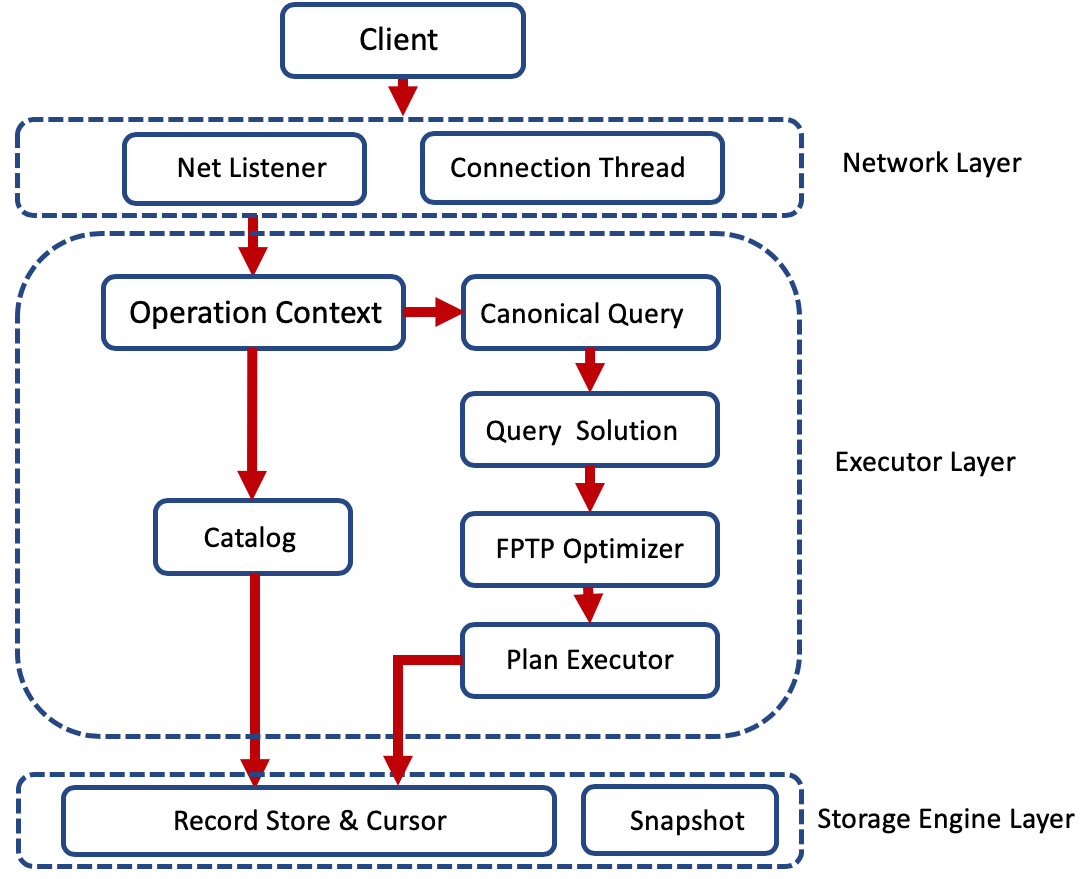
\includegraphics[width=0.9\linewidth]{images/body/overview.png}
  \caption{MongoDB query processing workflow.}
  \label{fig:workflow}
\end{figure}

At a low level, MongoDB stores data as BSON documents, which extends the JSON model to offer more data types and efficient encoding and decoding. APIs in a variety of programming languages make it easy for programmers to create those documents. This coupled with the similarity between MongoDB's JSON-like document model and the data structures used in object-oriented programming, makes integration with applications simple. 

MongoDB applications can use complex queries, secondary indexes, and aggregations to retrieve unstructured, semi-structured, and structured data. A vital factor in this flexibility is MongoDB's support for various query types. Queries can return documents, document projections, or complex aggregations calculated over
many documents \cite{mongodb_2019}.

% [Michael] this introduces range queries but not sure whether it's otherwise needed
\begin{description}
     \item[Key-value queries] Find documents where a field, usually the primary key, matches a given value.
     \item[Range queries] Find documents where field values match inequality predicates (e.g, greater than, less than or equal to, between).
     \item[Text search] Find documents in relevance order based on text arguments using Boolean operators such as AND, OR, NOT.
\end{description}

Here, we have a closer look at MongoDB's \verb|find()| query command and introduce
how it relates to SQL SELECT expressions.
%Example \ref{alg:findsyntex} shows the syntax of MongoDB \verb|find()| command.
\begin{lstlisting}[caption={MongoDB find() query example}, label={alg:queryexample}]
db.runCommand({
    "find": "movie",
    "filter": { 
        movieid: {"$gte": 0, "$lte":1000}, 
        avgrating: {"$gte": 5} 
    },
    "projection": {moviename: 1, avgrating: 1},
    "sort": {avgrating, -1},
    "limit": 10,
})
\end{lstlisting}

The most common operators for a \verb|find()| command are \verb|filter| (analogous to the SQL WHERE expression, with an implicit AND between conditions), \verb|projection| (analogous to the SQL SELECT expression) and \verb|sort|. MongoDB query is different from SQL in many ways: there is no complex semantic parsing, the query is written in BSON format (i.e. Binary~JSON, a binary form for representing simple or complex data structures, originated at MongoDB). Each operator in the query language corresponds to a field in a document that can be included or omitted as needed.

\subsection{Execution Plan Generation and Caching}

\begin{figure}[tb]
  \centering
  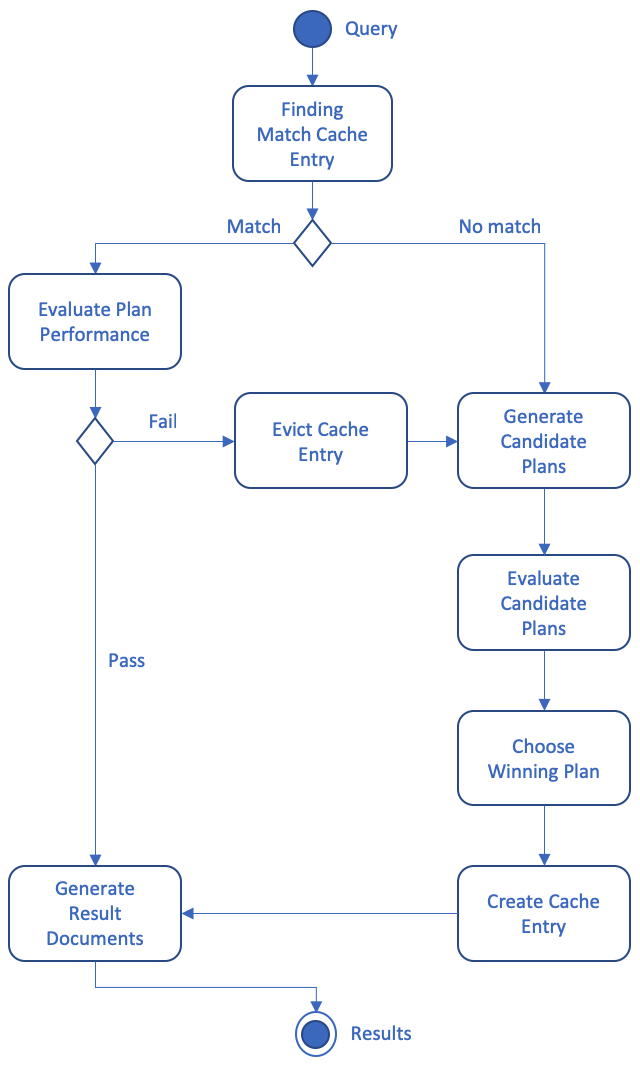
\includegraphics[width=0.75\linewidth]{images/background/query_planner_before.png}
  \caption{Logical flow of MongoDB query optimizer.}
  \label{figure:logicflow}
\end{figure}

The design of the MongoDB query processor and optimizer is evolving with each release. We provide detailed insight into the state-of-the-art architecture. The overall design of the optimizer is clean and orderly. However, in later sections we demonstrate that there is room for further improvement.

In this section, we explain how a MongoDB query is submitted, parsed, and optimized before it interacts with the MongoDB storage engine. Explanations in this section are mainly gathered from interviews with professional MongoDB developers and from examining MongoDB source code.

Figure \ref{fig:workflow} provides an overview of the query processing workflow. We break down the whole process into three layers. In the network layer, MongoDB specifies a MongoDB Wire Protocol which is a simple socket-based, request-response-style protocol. Clients connect to the database following the protocol. In the executor layer, queries are received in the form of operation contexts. Some queries such as \verb|insert()| do not require optimization. Therefore, these queries interact directly with the storage engine.

Queries that require optimization are standardized and simplified to Canonical Queries, which MongoDB calls the ``query shape'':\footnote{\url{https://mongodb.com/docs/manual/reference/glossary/\#std-term-query-shape}}:
\begin{description}
\item[Query shape] A combination of query predicate, sort, projection, and collation. The query shape allows MongoDB to identify logically equivalent queries and analyze their performance.

For the query predicate, only the structure of the predicate, including the field names, are significant. The values in the query predicate are insignificant. Therefore, a query predicate \verb|{ type: 'food' }| is equivalent to the query predicate \verb|{ type: 'utensil' }| for a query shape.
\end{description}

The query shape is designed for the cache mechanism; generation and evaluation of query plans uses a complete query with concrete values. 

The process of generating a canonical query mainly involves match expression optimization. A match expression is an expression consisting of logical operations in the \verb|filter| operator. To optimize a match expression, MongoDB extracts all logical operators and constitutes an expression tree.  In this process, MongoDB optimizes the ordering of logical expressions and eliminates duplicates. The simplified expression tree can be used to filter records later. 

For a given Canonical Query, the Query Solution module might yield multiple execution plans. Each execution plan is a tree of query stages, where the leaf stages access data via a collection or index. When there are multiple relevant indexes, execution plans are generated to explore the combinations. Multiple execution plans will also be generated when stages can be reordered or there are multiple implementations of a given stage (e.g., \verb|$or| queries and joins expressed with \verb|$lookup|).

All candidate execution plans are evaluated by the \approachName query optimizer. Finally, the candidate plan assigned the best efficiency score by \approachName is executed by the plan executor. The plan is also cached, and if the same query shape is executed soon after, the cached plan will be reused as long as its efficiency remains below 10 times the evaluated efficiency (with default settings).

% [Michael] I've replaced the following
\begin{comment}
\af{I don't understand the following two sentences; in general, can't there be multiple plans that differ in ways other than choice of index?} During optimization, if more than one index is associated with the plan, multiple candidate execution plans are considered. Otherwise, only one execution plan is generated. All candidate execution plans are evaluated by the \approachName query optimizer. Finally, the candidate plan assigned the best efficiency score by \approachName is executed by the plan executor. The plan is also cached, and if the same query shape is executed soon after, the cached plan will be used without considering alternatives.

% TODO  [Hash: Do we really need this part? It's just introducing search commands...]

\begin{procedure}[ht]
    \caption{MongoDB find() command syntax}
    \begin{verbatim}
    db.runCommand(
       {
          "find": <string>,
          "filter": <document>,
          "sort": <document>,
          "projection": <document>,
          "hint": <document or string>,
          "skip": <int>,
          "limit": <int>,
          "batchSize": <int>,
          "singleBatch": <bool>,
          "comment": <string>,
          "maxTimeMS": <int>,
          "readConcern": <document>,
          "max": <document>,
          "min": <document>,
          "returnKey": <bool>,
          "showRecordId": <bool>,
          "tailable": <bool>,
          "oplogReplay": <bool>,
          "noCursorTimeout": <bool>,
          "awaitData": <bool>,
          "allowPartialResults": <bool>,
          "collation": <document>
       }
    )
    \end{verbatim}
    \label{alg:findsyntex}
\end{procedure}

\begin{lstlisting}[caption={MongoDB find() query example}, label={alg:queryexample}]
db.runCommand({
    "find": "movie",
    "filter": { 
        movieid: {"$gte": 0, "lte":1000}, 
        avgrating: {"gte": 5} 
    },
    "projection": {moviename: 1, avgrating: 1},
    "sort": {avgrating, -1},
    "limit": 10,
})
\end{lstlisting}

% [Michael] ideally this would be the query shape for the example movie query given above
\af{I am confused; these seem to have explcit constants, unlike what a query shape should be. Also, I agree with Michael that it would be clearer to give simply one shape, which would be for the query in Listing 1}

\begin{lstlisting}[caption={Examples of query shape}, label={alg:queryshape}]
[
    {
        "query" : { "qty" : { "$gt" : 10 } },
        "sort" : { "ord_date" : 1 },
        "projection" : { },
        "queryHash" : "9AAD95BE" 
    },
    {
        "query" : { "$or" :
           [
             { "qty": { "$gt" : 15}, "item" : "xyz123"},
             { "status" : "A" }
           ]
        },
        "sort" : { },
        "projection" : { },
        "queryHash" : "0A087AD0"  
    },
    {
        "query" : { "$or" : 
            [ 
                { "qty" : { "$gt" : 15 } },
                { "status" : "A" }
            ]
        },
        "sort" : { },
        "projection" : { },
        "queryHash" : "DA43B020"
    }
]
\end{lstlisting}

\subsubsection{Canonical Query} \label{sec:canonical-query}
\end{comment}

% [Michael] TODO check whether we end up including results evaluating the effect of the query cache and update the following:
In this work, we mainly focus on investigating the query optimizer's query plan evaluation strategy but not the efficiency of its cache mechanism. In the experimental analysis, we programmatically force MongoDB not to use the query plan cache. 

\subsection{MongoDB's \approachName Query Optimizer}

\begin{comment} Michael: I've rewritten the pseudocode to match the implementation and updated the description to match. How does it look now?
\af{I found the description and code not well matched. advanced is a counter not a return value, and the text doesn't explain how isEOF is modified. Can Michael check this. Also code should I think say advanced greater or equal MaxResults, rather than less than.}
\end{comment}

\begin{comment} Michael's notes
For future references, \ref{alg:es} is summarising the code in src/mongo/db/exec/multi_plan.cpp, specifically the main loops in MultiPlanStage::pickBestPlan and MultiPlanStage::workAllPlans.
\end{comment}

\begin{algorithm}[tb]
    \caption{Algorithm used for early termination of the simulation}
    \begin{algorithmic}
        \REQUIRE $collection$, the main data source for the query, and $candidates$, a list of candidate plans
        \ENSURE statistics describing each plan's trial execution
        \STATE $maxWorks \gets max(10000, 0.3 * numRecords(collection))$
        \STATE $maxResults \gets 101$ \COMMENT{with default configuration}
        \STATE $working \gets$ \TRUE
        \STATE $i \gets 0$
        \STATE $plan.results \gets 0$ $\forall$ $plan \in candidates$
        \STATE
        \WHILE{$working$ \AND $i < maxWorks$}
            \FORALL{$plan \in candidates$}
                \STATE $state \gets plan.work()$
                \IF{$state$ = ADVANCED}
                    \STATE $plan.results \gets plan.results + 1$
                    \IF{$plan.results \ge maxResults$}
                        \STATE $working \gets$ \FALSE
                    \ENDIF
                \ELSIF{$state$ = EOF}
                    \STATE $working \gets$ \FALSE
                \ENDIF
            \ENDFOR
            \STATE $i \gets i + 1$
        \ENDWHILE
    \end{algorithmic}
    \label{alg:es}
\end{algorithm}

We now describe the mechanism of MongoDB's query optimizer. A simplified explanation of \approachName is that the query optimizer initially executes all potential query plans in parallel and chooses the first one that completes a predefined amount of work. The winner of the race is then run to completion as the execution plan and is also cached for future queries with the same shape. 

The \approachName approach consists of two key steps: measuring all candidate plans in a race and then making a decision, that is, choosing the most efficient query plan based on the measurements. During the race phase, all candidate query plans are executed in a round-robin fashion. That is, MongoDB starts all candidate query plans and cycles through them to simulate the execution of the query. During the simulation, time slices are assigned to each query plan in equal portions and in circular order, handling all potential plans. Meanwhile, the query optimizer gathers execution metrics and then provides a score for each plan. 

The query optimizer asks each plan for the next document, via a call to a \verb|work()| function. If the plan can provide a document, it responds with \verb|ADVANCED|. If all documents from the plan have been retrieved, \verb|work()| returns \verb|EOF| and \verb|working| is set to \verb|false|. However, the given query could be expensive, so MongoDB specifies limits to terminate the simulation early, as described in Algorithm \ref{alg:es}.

The simulation stops if the maximum allowable amount of work has been reached, or the requested number of documents has been retrieved (as reflected in the counter $plan.results$), or a plan has completed and returned all its results. The configuration knob $internal\-Query\-Plan\-Evaluation\-Works$ (default 10,000) is the maximum allowed amount of work. However, for very large collections, MongoDB takes a fraction of the number of documents to determine the maximum allowable amount of work. The configuration knob $internal\-Query\-Plan\-Evaluation\-Max\-Results$ (default 0.3) is the maximum number of documents that can be retrieved during the simulation.

\begin{table}[htb]
    \begin{tabular}{ll}
        \toprule
        Metric         & Value\\
        \midrule
        baseScore      & 1                                           \\
        Productivity   & queryResults / workUnits                    \\
        TieBreak       & min(1.0 / (10 * workUnits), 1e-4)           \\
        noFetchBonus   & TieBreak or 0                               \\
        noSortBonus    & TieBreak or 0                               \\
        noIxisectBonus & TieBreak or 0                               \\
        tieBreakers    & noFetchBonus + noSortBonus + \\
                       & noIxisectBonus \\
        eofBonus       & 0 or 1\\
        \bottomrule
    \end{tabular}
    \caption{MongoDB Query Plan Performance Metrics}
    \label{table:pm}
\end{table}

When the simulation ends, each candidate query plan is assigned a performance score based on the performance metrics shown in \autoref{table:pm}. The query optimizer chooses the query plan that has the highest performance score as the execution plan. The performance score is calculated as:
\begin{align}
 score = baseScore + productivity + tieBreakers + eofBonus
\end{align}

Each query plan has a base score of 1. The $productivity$ of a plan is measured as the number of results returned divided by the total amount of work performed. $tieBreakers$ is a very small bonus number that is given when a plan contains no fetch operation ($noFetchBonus$), no blocking sort ($noSortBonus$) or avoids index intersection ($noIxisectBonus$). $eofBonus$ is given if all possible documents are retrieved during the execution of the plan.